\documentclass{article}
\setlength{\parindent}{0pt}
\usepackage[spanish]{babel}
\usepackage{colortbl}
\usepackage{graphicx}
\usepackage{listings}
\usepackage{minted}
\setminted{%
  breaklines=true,
  autogobble=true,
  bgcolor=yellow,
  fontsize=\footnotesize,
  frame=lines,
  framesep=2mm,
  baselinestretch=1.2,
  linenos
}
\newminted{bash}{%
    linenos,
    autogobble,
    frame=lines,
    framesep=2mm,
    baselinestretch=1.2,
    fontsize=\footnotesize,
    mathescape,
    breaklines % <-- Agrega esta opción
}
% Definir el entorno para el código de shell
\lstnewenvironment{shell}{%
  \lstset{%
    language=bash,
    basicstyle=\ttfamily,
    breaklines=true,
    columns=fullflexible
  }
}{}
% Set page size and margins
\usepackage[letterpaper,top=2cm,bottom=2cm,left=3cm,right=3cm,marginparwidth=1.75cm]{geometry}

\begin{document}

\thispagestyle{empty}
\begin{titlepage}
\centering
\begin{center}
\begin{tabular}{c c}

\includegraphics[width=0.25\textwidth]{gg.png}\hspace{5cm}&\hspace{6cm}
\includegraphics[width=0.25\textwidth]{download.png}\\
\end{tabular}
\end{center}

{\scshape\LARGE Universidad Nacional Autónoma de México \par}
\vspace{2cm}
{\scshape\Large Programa de Tecnología y Cómputo \par}
{\scshape\Large GNU/Linux \par}
\vspace{2cm}
{\scshape\Large Proyecto: \par}
{\Large Terminal de trabajo \par}
\vfill
{\scshape\Large Buddys: \par}
{\Large Leonardo Demián González Zamaora \par}
{\Large Dulce Michelle Barrios Aguilar \par}

\vfill
{\Large Generación 45º\par}
\vfill
{\Large 22 de septiembre, 2023 \par}
\end{titlepage}
%=======================================================================================
\newpage
\color{black}
\tableofcontents
\newpage 
\section*{Introducción}
\addcontentsline{toc}{section}{Introducción}
Un sistema operativo es un programa que administra y gestiona eficientemente los recursos de una computadora, buscando la seguridad, estabilidad y robustez. En nuestro campo, la gestión eficiente de sistemas es fundamental para mejorar la productividad.\\

GNU/Linux nos ofrece un núcleo completo y funcional que administra los recursos a nivel de hardware y su filosofía de código abierto es ampliamente adoptada en entornos laborales, lo que hace que el proyecto GNU/Linux sea amigable y compatible con nuestras necesidades.\\

El término "Shell" hace referencia al intérprete de comandos que permite a los usuarios interactuar con el sistema operativo y ejecutar comandos. Durante nuestro curso, aprendimos que al ingresar comandos en la shell, que en Linux es llamada Bash, podemos realizar diversas tareas.\\

En este proyecto, ambos buddys creamos una terminal de trabajo basada en Shell Script, lo que nos permite aplicar nuestros conocimientos adquiridos en el curso además de demostrar nuestra capacidad de investigación para cumplir con el objetivo de diseñar una interfaz de usuario con características únicas.\\

Hemos logrado una solución eficiente para una terminal de comandos personalizada que se centra en la automatización de tareas y la flexibilidad que ofrece Shell Script con nuestro toque.\\

La terminal de trabajo mostrada a continuación permite a los usuarios trabajar con archivos mediante comandos personalizados que facilitan la consulta de información del sistema, la reproducción de música y la inclusión de juegos que está diseñada para ser eficiente y fácil de usar, ya que los comandos implementados son intuitivos y fáciles de recordar.  

\newpage
\section*{Desarrollo}
\addcontentsline{toc}{section}{Desarrollo}
Para la realización de este proyecto,ambos buddys discutimos los objetivos y dimos propuestas a la solución para llevar el trabajo colaborativo de la mejor manera no solo para la parte opertaiva, sino también de las características visules que se buscaban implementar.\\

Decidimos trabajar remotamente con los scripts que nos llamaran la atención por lo que se tuvo la siguiente forma de trabajo:

\subsection*{Repositorio en GitHub del Proyecto Linux}
\addcontentsline{toc}{subsection}{Repositorio en GitHub del Proyecto Linux}
La creación de un repositorio en GitHub era un requerimiento en el proyeccto, ya que se busca ver la evidencia de que ambos buddys estuvieron involucrados en el proyecto, sin embargo,inicialmente cada uno de nosotros trabajo en su propio repositorio, por lo que faltando pocos días para la entrega se decidió "migrar" al repositorio que estaba mas avanzado.

Michelle tuvo que realizar el fork del repositorio de Leonardo para comenzar a trabajar, y Leonardo tuvo que aceptar los cambios, los pull request para que se vean reflejados los commits, es decir, todos los cambios que se iban realizando durante la realización del proyecto.

\begin{figure}[ht]
\centering
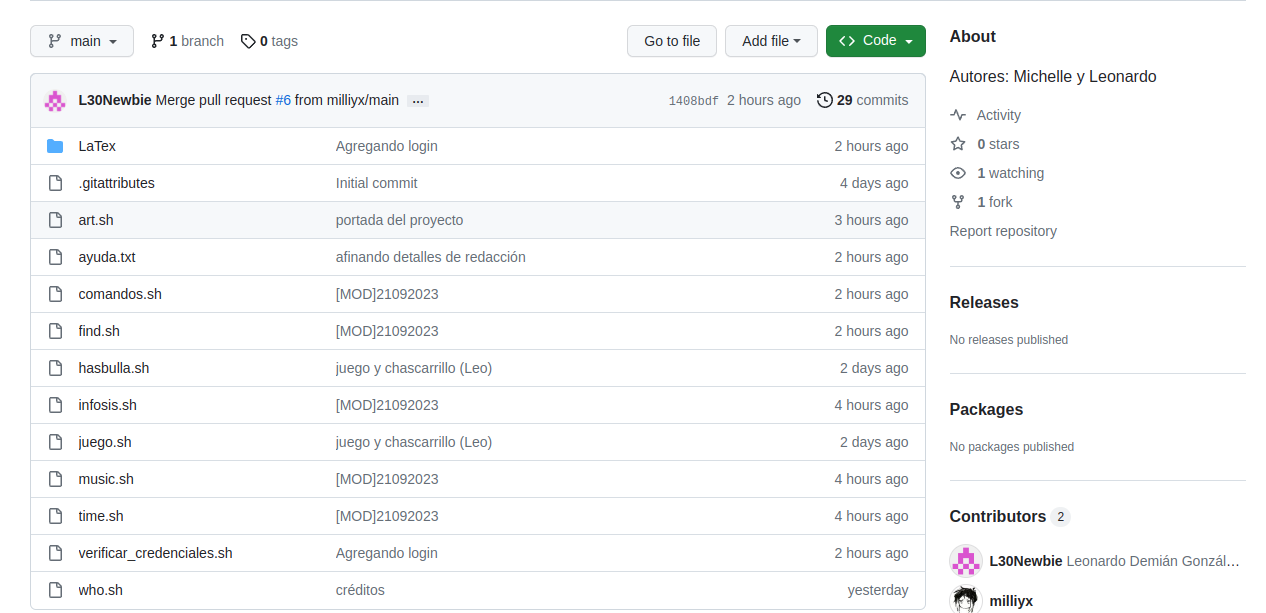
\includegraphics[width=1\textwidth]{cap1.png}
\caption{\label{fig:frog1}Repositorio en GitHub del Proyecto Linux}
\end{figure}

\subsection*{Scripts a utilizar}
\addcontentsline{toc}{subsection}{Scripts a utilizar}
Las especificaciones en el proyecto nos dice que es lo que puede o debe realizar la terminal de trabajo , por lo que se definieron los siguientes scripts:

\begin{enumerate}
\item \textit{art.sh}\\
Script que muestra arte ASCCII
\\
\item \textit{comandos.sh}\\
Script que ayuda a ejecutar scripts como comandos así como comandos ya existentes en el sistema operativo.
\\
\item \textit{find.sh}\\
Script que pueda buscar un archivo en un directorio específico
\\
\item \textit{hasbulla.sh}\\
Script que muestra arte ASCCII
\\
\item \textit{infosis.sh}\\
Script que muestra información del sistema.
\\
\item \textit{juego.sh}\\
Script que despliega un juego, en nuestro caso Ahorcado.
\\
\item \textit{music.sh}\\
Script que despliega una interfaz gráfica de un reproductor mp3.
\\
\item \textit{time.sh}\\
Script que muestra fecha y hora.
\\
\item \textit{ayuda.txt}\\
Script que muestra una lista de comandos disponibles y una breve descripción. 
\\
\item \textit{verificar}\textunderscore \textit{credenciales.sh}\\
Sistema de acceso inicial para los usuarios.
\\
\item $who.sh$\\
Script que muestra los créditos de ambos buddys.
\end{enumerate}

\subsection*{Compilación del Proyecto Linux}
\addcontentsline{toc}{subsection}{Compilación del Proyecto Linux}

 Como ambos buddys tenemos acceso en tiempo real a los archivos modificados y/o agregados en el repositorio, nos resultó fácil realizar pruebas que nos indicará el correcto funcionamiento del proyecto. \\
 
 Para ejecutar el programa se escribe el siguiente comando que, como lo aprendimos en el curso, se utiliza para otorgar permisos de ejecución a un archivo o directorio a todos los usuarios. El comando a utilizar tiene la siguiente sintáxis:
\begin{verbatim}
chmod +x comandos.sh art.sh find.sh hasbulla.sh infosis.sh juego.sh time.sh ...
\end{verbatim}

En donde tenemos que poner el nombre de cada uno de los scripts que son utilizados en el programa con su respectiva extensión para el correcto funcionamiento de la terminal de trabajo. \\

En seguida, para ejecutar el programa, se sigue la siguiente sintáxis:
\begin{verbatim}
./verificar_credenciales.sh comandos.sh art.sh find.sh hasbulla.sh infosis.sh ...
\end{verbatim}
\begin{figure}[ht]
\centering
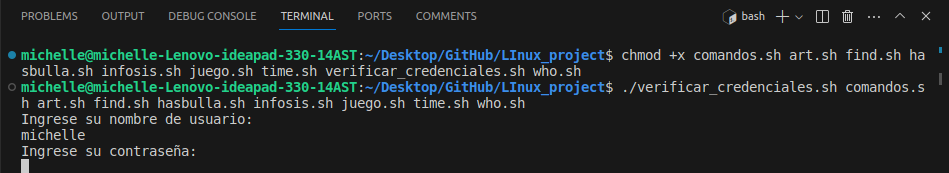
\includegraphics[width=1\textwidth]{cap3.png}
\caption{\label{fig:frog2}Compilación del Proyecto Linux}
\end{figure}

\subsection*{Ejecución del Proyecto Linux}
\addcontentsline{toc}{subsection}{Ejecución del Proyecto Linux}

Inicialmente, se ejecuta el archivo \textit{verificar}\textunderscore \textit{credenciales.sh} que muestra el sistema de acceso para los usuarios, siendo éste el primer elemento que se muestra en pantalla.\\

Se requiere que el usuarion ingrese usuario y contraseña, cabe recalcar que estos datos deberán existir en el sistema operativo anfitrión, de lo contrario, si las credenciales no coinciden no tendran acceso a la terminal de trabajo. \\

Para esta parte,hacemos uso del script \textit{verificar\textunderscore credeciales.sh}. 
\begin{figure}[ht]
\centering
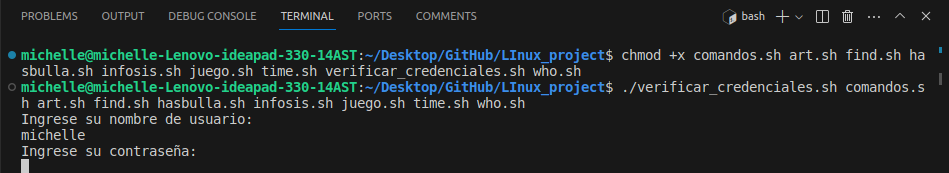
\includegraphics[width=1\textwidth]{cap3.png}
\caption{\label{fig:frog3} Sistema de acceso. Usuario.}
\end{figure}

\begin{bashcode}
# Verificar si el usuario existe
if ! id "$username" &>/dev/null; then
  echo "Usuario inválido"
  exit
fi

if [[ $(passwd -S "$username" | awk '{print $2}') == "P" ]]; then
  echo "Ingrese su contraseña:"
  read -s password
  pass=1
  if ! echo "$password" | su - "$username" -c 'echo ""' >/dev/null 2>&1; then
    echo "Contraseña incorrecta"
    pass=0
  fi
else
  echo "La contraseña para el usuario $username está inactiva"
  pass=0
fi
\end{bashcode}

Este extracto de codigo verifica si el usuario existe y si su contraseña es correcta.

\begin{verbatim}
if [[ $(passwd -S "$username" | awk '{print $2}') == "P" ]]; then
\end{verbatim}

Mediante el comando \textbf{psswd -S}, comando que pertenece a la bash del SO, verifica si la contraseña del usuario está activa.\\

Si el usuario existe y la contraseña está activa, se le pide al usuario que ingrese su contraseña mediante \textbf{read -s}.
\begin{verbatim}
if ! echo "$password" | su - "$username" -c 'echo ""' >/dev/null 2>&1; then
\end{verbatim}

Se usa el comando \textbf{su} para verificar si la contraseña ingresada es correcta para imprimir un mensaje de bienvenida, si no lo es se imprime un mensaje de error. \\

\begin{figure}[ht]
\centering
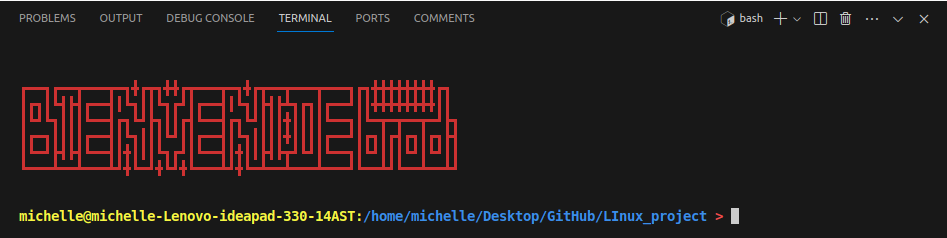
\includegraphics[width=1\textwidth]{cap2.png}
\caption{\label{fig:frog6} Mensaje de bienvenida al usuario}
\end{figure}

Una vez que estamos dentro de la terminal de trabajo que personalizamos se muestra el mensaje de bienvenida y tal como lo dicen los requerimientos del proyecto, debe existir una lista de comandos para que el usuario pueda interactuar con la terminal. 

\subsection*{Script comando}
\addcontentsline{toc}{subsection}{Script comando}
El script nos ayuda a crear la shell interactiva a través de un menú de opciones en el que se obtiene el nombre de usuario y su directorio actual.\\

\begin{bashcode}
while true; do
    usuario=$(whoami)
    ruta_actual=$(pwd)
\end{bashcode}

Muestra el PROMPT con colores específicos y una flecha simulando la terminal de Linux que muestra el nombre de usuario activo así como la carpeta donde se encuentran.\\

\begin{bashcode}
        # Mostrar el prompt simulado con colores y flecha
    echo -ne "${color_usuario}$usuario@$(hostname):${color_ruta}$ruta_actual${flechita} > ${color_reset}"

    read -p "" opcion
\end{bashcode}

Además, lee la opción del usuario mediante un \textit{case} para manejar las distintas opciones que representan los comandos que ejecutan un script en específico. \\

A pesar de ser una terminal personalizada, conserva la capacidad de interpretar no solo los comandos que nostros definimos, sino, los del SO anfitrión. Esto lo puede realizar tratando el valor de \textit{opcion} como un comando del SO, y lo ejecuta como si se hubera ingresado en la línea de comandos del SO.

\begin{bashcode}
            *)
            # Si la opción no está en el menú, intentar ejecutarla como comando del sistema
            $opcion
            ;;
\end{bashcode}

\newpage
\subsection*{Comando ayuda}
\addcontentsline{toc}{subsection}{Comando ayuda}

El comando ayuda nos muestra una serie de comandos definidos por nostros para que el usuario interactúe con nuestra terminal, no es un script como tal, sino, un archivo de texto.\\

\begin{figure}[ht]
\centering
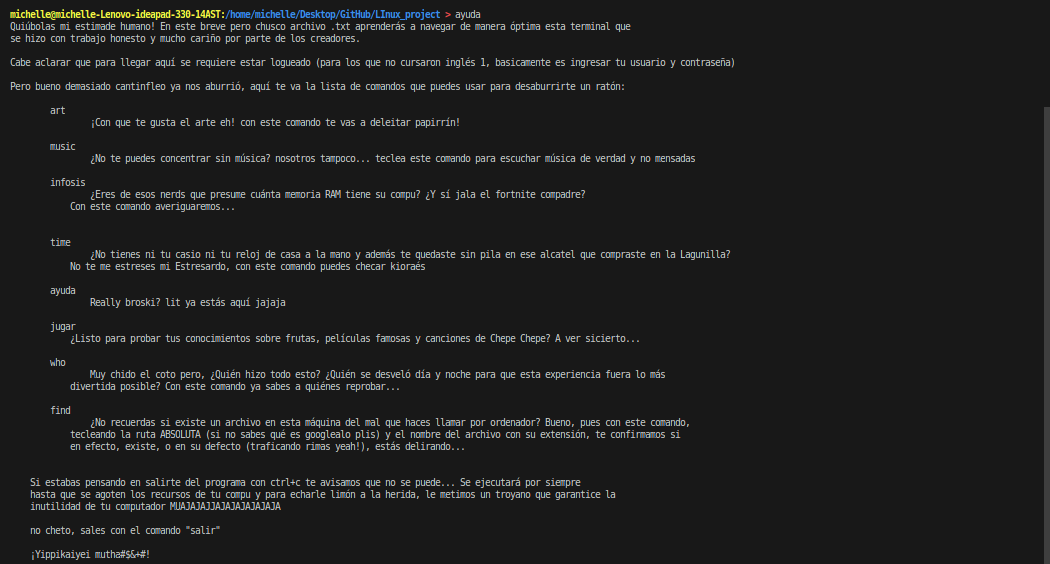
\includegraphics[width=1\textwidth]{cap4.png}
\caption{\label{fig:frog4} Comando ayuda}
\end{figure}

\newpage
\subsection*{Comando music}
\addcontentsline{toc}{subsection}{Comando music}

Este comando despliega una interfaz gráfica que permite formas de navegar sobre la biblioteca musical, permitiendo la visualización de la canción, cambiar entre canciones, pausar, reaunudar, etc. \\

\begin{bashcode}
    # Solicitar al usuario la ruta de la biblioteca musical
MUSIC_DIR=$(zenity --file-selection --directory --title="Selecciona la carpeta de tu biblioteca musical")

# Verificar si mpg123 está instalado
if ! command -v mpg123 &>/dev/null; then
  zenity --question --text="El reproductor mpg123 no está instalado. ¿Desea instalarlo?" --title="Reproductor MP3"

  if [ $? -eq 0 ]; then
    # Instalar mpg123 (debes proporcionar el comando de instalación adecuado según tu sistema)
    sudo apt-get install mpg123  # Ejemplo para sistemas basados en Debian
  else
    zenity --error --text="Reproductor MP3 no disponible. Saliendo." --title="Reproductor MP3"
    exit 1
  fi
fi
\end{bashcode}

Utiliza el programa \textbf{mpg123} para la reproducción de archivos MP3.\\

Mediante \textbf{utilidad zenity} solicita al usuario ruta de biblioteca musical y verifica si el programa mpg123 está instalado, si no lo está se le pide al usuario que lo intale, en modo super usuario. 


\begin{figure}[ht]
\centering
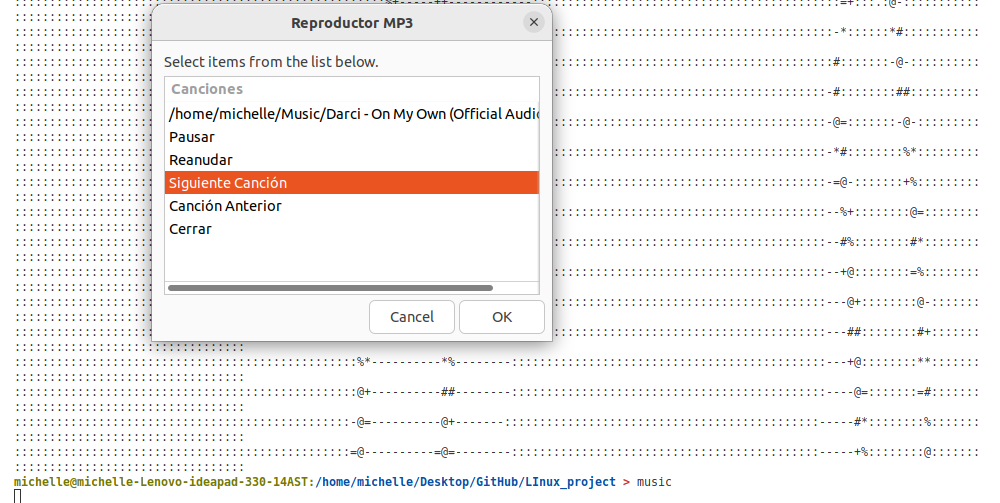
\includegraphics[width=1\textwidth]{cap6.png}
\caption{\label{fig:frog7} Comando music}
\end{figure}

\subsection*{Script infosis}
\addcontentsline{toc}{subsection}{Script infosis}

En este script se obtiene la información requerida por medio del comando \textbf{awk} que es un comando del SO anfitrión se utiliza para leer el archivo \textbf{proc/meminfo} para obtener la cantidad total de RAM del sistema para después almacenar este dato en una variable \textbf{mem \textunderscore total} e imprimirlo mediante un \textbf{echo}.\\

El comando \textbf{uname} que también pertenece al SO, obtiene la arquitectura del sistema por lo que se sigue el mismo proceso de alamacenar dicho dato en una variable e imprimirlo mediante \textbf{echo}.\\

Mediante el comando \textbf{cat} perteneciente al SO, lee el archivo \textbf{/etc/os-release} y con \textbf{grap} busca la línea que contiene la versión del SO del usuario para imprimirlo con un \textbf{echo}.
\begin{bashcode}
    # Obtener información de la memoria RAM
echo -e "\e[36mMemoria RAM:\e[0m"
mem_total=$(awk '/MemTotal/ {print $2}' /proc/meminfo)
mem_total_mb=$(echo "scale=2; $mem_total / 1024" | bc)
echo -e "Total de memoria RAM: \e[35m$mem_total_mb MB\e[0m"

# Obtener la arquitectura del sistema
echo -e "\n\e[36mArquitectura del sistema:\e[0m"
arch=$(uname -m)
echo -e "Arquitectura: \e[35m$arch\e[0m"

# Obtener la versión del sistema operativo
echo -e "\n\e[36mVersión del sistema operativo:\e[0m"
os_version=$(cat /etc/os-release | grep "VERSION=" | cut -d '"' -f 2)
echo -e "Versión del sistema operativo: \e[35m$os_version\e[0m"
\end{bashcode}

\subsection*{Script time}
\addcontentsline{toc}{subsection}{Script time}

\textbf{TZ} especifica la zona horaria del sistema y mediante comando \textbf{date} que pertenece al SO obtiene la fecha y hora actuales en formato año-mes-dia. 

\begin{bashcode}
# Guardar el valor actual de TZ
OLD_TZ=$TZ

# Configurar la zona horaria a UTC (o la que prefieras)
TZ=UTC

# Obtener la fecha actual en la zona horaria configurada
fecha_actual=$(date +"%Y-%m-%d")
\end{bashcode}

\begin{figure}[ht]
\centering
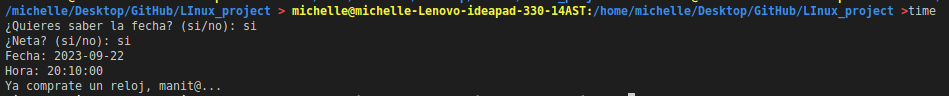
\includegraphics[width=1\textwidth]{cap7.png}
\caption{\label{fig:frog8} Comando time}
\end{figure}

\newpage
\subsection*{Script jugar}
\addcontentsline{toc}{subsection}{Script jugar}

Este script ejecuta un juego de ahorcado donde el jugador debe adivinar una palabra de una categoría elegida al azar. El juego tiene 7 intentos y el jugador gana si adivina la palabra antes de que se agoten los intentos.

\begin{figure}[ht]
\centering
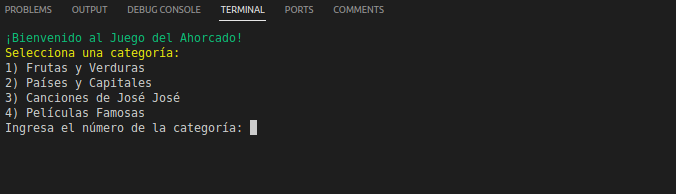
\includegraphics[width=1\textwidth]{cap8.png}
\caption{\label{fig:frog9} Comando juego}
\end{figure}

\subsection*{Script who}
\addcontentsline{toc}{subsection}{Script who}

Este comando muestra los creditos de los creadores de este proyecto, Leonardo y Michelle, jugando con los colores y tipografías usando el arte ASCII.

\begin{figure}[ht]
\centering
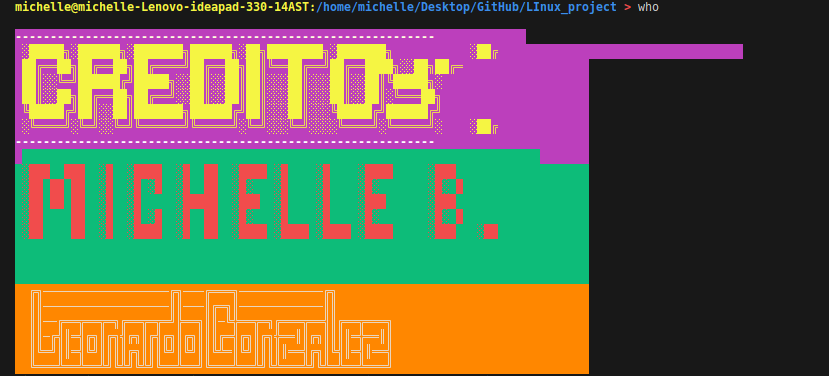
\includegraphics[width=1\textwidth]{cap5.png}
\caption{\label{fig:frog10} Comando who}
\end{figure}
\subsection*{Script find}
\addcontentsline{toc}{subsection}{Script find}

Este comando pide al usuario la ruta absoluta y el nombre de un archivo para comprobar si existe o no mediante una concatenación: 

\begin{bashcode}
ruta_completa="$ruta_archivo/$nombre_archivo"
\end{bashcode}

Después verifica si el archivo exite e imprime un mensaje de confimación o de error según sea el caso.

\begin{bashcode}
if [ -e "$ruta_completa" ]; then
  echo "En efecto, este archivo existe mi panamá. ;)"
else
  echo "Pa mí que te lo estás inventando mi tibio -_-"
fi
\end{bashcode}

\begin{figure}[ht]
\centering
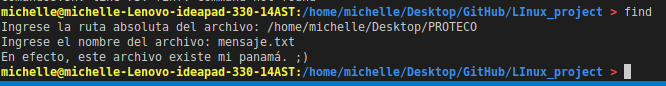
\includegraphics[width=1\textwidth]{cap9.png}
\caption{\label{fig:frog11} Comando find}
\end{figure}

\section*{Conclusiones}

\addcontentsline{toc}{section}{Conclusiones}

\subsection*{Leonardo Demián González Zamaora}
\addcontentsline{toc}{subsection}{Leonardo Demián González Zamaora}

Sin duda alguna, fue un proyecto interesante e intimidante a la vez, aunque sea para mí. Desde un principio dudé si era algo que podía hacer, pero con el tiempo, fue algo que fui perdiendo con la ayuda de investigación y apoyo constante de mi buddy.\\

Disfruté mucho el trabajo en equipo con Michelle porque nos supimos comunicar de manera efectiva en todo momento, siendo honestos y transparentes con nuestro avances.\\

Al final, el resultado me agradó bastante y estoy contento con el desempeño que tuvimos como equipo.\\

\subsection*{Dulce Michelle Barrios Aguilar}
\addcontentsline{toc}{subsection}{Dulce Michelle Barrios Aguilar}

Al realizar la lectura del documento en donde se presentaban los requerimientos, pensé que iba a ser imposible hacer un proyecto así con los conocimientos básicos de Shell Script. Gracias a la investigación que se realizó junto a mi buddy pudimos sacar adelante este proyecto a base de la comunicación constante que se tuvo para lograrlo.

La parte que mas me gustó del proyecto fue la personalización de la terminal, y claro, como existen funciones en las cuales podemos tomar información de los comandos ya existentes en SO anfitrión para poder hacer los propios, pero no tan fácil con copiar dicha información e imprimirla, si no, aplicándolo de una manera lógica mediante el código.

Sin duda a Leonardo y a mi nos llevo bastante tiempo y bastantes pruebas para que quedara como queríamos, pero de mi parte, estoy satisfecha con los conocimientos adquiridos durante el desarrollo del proyecto y por la experiencia de haber creado una terminal de trabajo en Bash Shell Script. 

\end{document}
